\documentclass[border=0pt]{standalone}
\usepackage{tikz}
\usepackage{amsmath}
\usepackage{pgfplots}
\pgfplotsset{width=\linewidth,compat=1.8}
\begin{document}

\tikzstyle{every node}=[font=\bfseries\Huge]
\pgfplotsset{every tick label/.append style={font=\boldmath\Huge}}
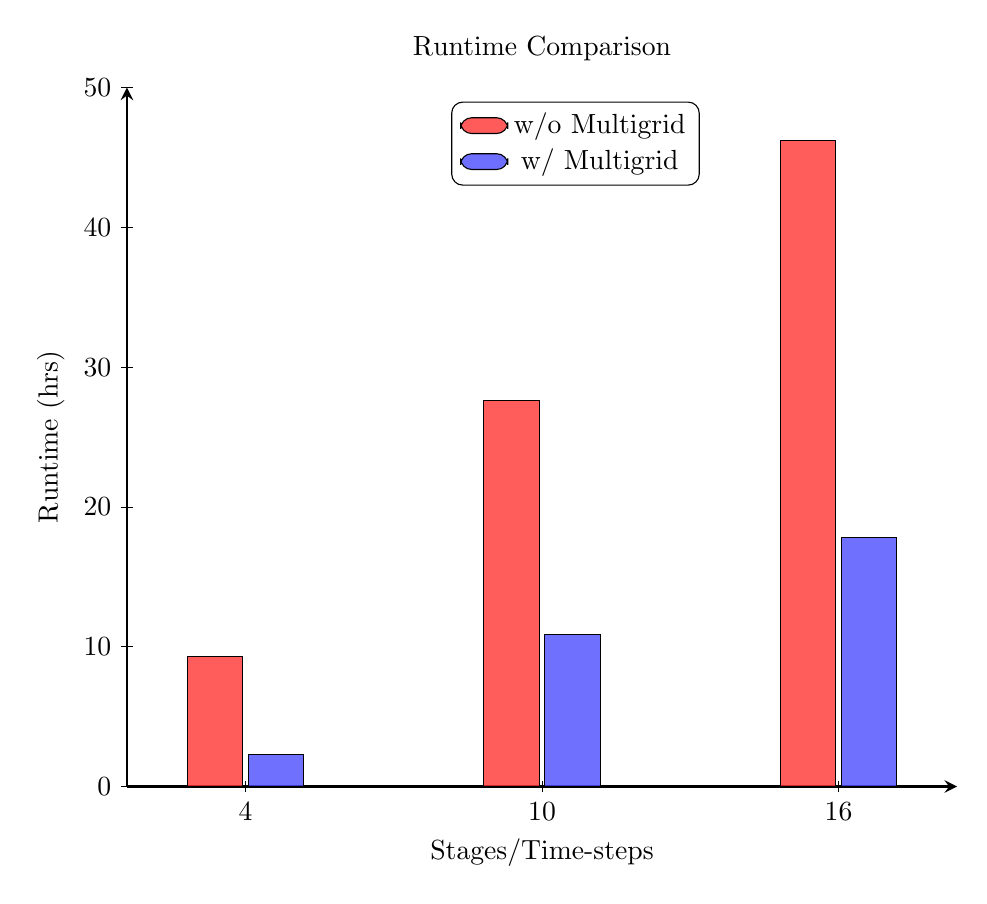
\begin{tikzpicture}
\begin{axis}[
    % width=10cm,
    % height=7cm,
    ybar,
    bar width=20pt,
    % symbolic x coords={4,10,16},
    % symbolic y coords={0, 10, 20, 40},
    ytick={0, 10, 20, 30, 40, 50},
    xtick=data,
    ymin=0,
    ymax=50,
    axis line style={line width=1pt},
    axis lines=left,
    clip=false,
    enlarge x limits=0.2,
    legend image code/.code={
            \draw[#1] (0cm,-0.1cm) rectangle (0.6cm,0.1cm);
        },
    legend style={
        at={(0.69,0.98)},
        anchor=north east,
        draw=black,
        fill=white,
        rounded corners,
        legend image post style={only marks},
        % text depth=0pt,
        % text height=1.5ex,
    },
    xlabel={Stages/Time-steps},
    ylabel={Runtime (hrs)},
    axis line style={black},
    tick style={black},
    every axis plot/.append style={fill opacity=0.8},
    % Add box around plot
    axis on top=false,
    % box plot=false,
    % title style={font=\bfseries},
    title={Runtime Comparison},
]
\addplot[fill=red!80] coordinates {
    (4,9.3)
    (10,27.6)
    (16,46.21)
};

\addplot[fill=blue!70] coordinates {
    (4,2.32)
    (10,10.9)
    (16,17.83)
};
\legend{w/o Multigrid, w/ Multigrid}
\end{axis}
\end{tikzpicture}

\end{document}
